\documentclass{beamer}
\usetheme{Goettingen}
\usefonttheme[onlymath]{serif}

\usepackage[version=4]{mhchem}
\usepackage{graphicx}
\usepackage{svg}
\usepackage{empheq}
\usepackage[many]{tcolorbox}

\usefonttheme{professionalfonts}
\usepackage{times}
\usepackage{amsmath}
\usepackage{verbatim}

\usepackage{tikz}
\usetikzlibrary{arrows,shapes,positioning,shadows,trees,matrix}
\tikzset{>=stealth}
\newcommand{\tikzmark}[3][]{\tikz[remember picture,baseline] \node [anchor=base,#1,](#2) {#3};}

\definecolor{red1}{RGB}{255,0,0}
\definecolor{red2}{RGB}{190,0,190}
\definecolor{red3}{RGB}{40,0,210}
\tcbset{highlight math style={enhanced, colframe=blue!20!black, colback=white, arc=4pt, boxrule=0.5pt}}

\title[Molecular Hydrophobicity Potential]
{%
    Implementing Molecular Hydrophobicity Potential Measurment for the Analysis of Dynamic Biomolecular Interactions
}
\date{\today}
\author[Pelg Bar Sapir]
{
    Peleg Bar Sapir\inst{1} \and \\
    Under supervision of Prof. Maria Andrea Mroginski\inst{2}
}
\institute[Freie Universit\"{a}t Berlin, Techniche Universit\"{a} Berlin]
{
    \inst{1}%
        Freie Universit\"{a}t Berlin
    \and
    \vskip-2mm
    \inst{2}%
        Techniche Universit\"{a}t Berlin
}

\begin{document}
\tikzstyle{every picture}+=[remember picture]
\everymath{\displaystyle}

\begin{frame}
    \titlepage
\end{frame}

\begin{frame}{Outline}
    \tableofcontents
\end{frame}

\section{Introduction}
\subsection{Hydrophobicity and log P}

\section{Molecular Hydrophobicity Potential}
\subsection{Potential}
\subsubsection{General form}

\begin{frame}{The MHP Formula}

    \centering
    \includesvg[scale=0.1]{mhp_visual1}

    \begin{equation*}
        \text{MHP}\left(\mathbf{x'}\right)=
        \tikz[baseline]{
            \node[anchor=base] (sum)
            {$\sum_{i=1}^{k}\limits$};
        }\left[ 
        \tikz[baseline]{
            \node[anchor=base] (force)
            {$f_i$};
        } \cdot
        \tikz[baseline]{
            \node[anchor=base] (distance)
            {$D\left(\mathbf{x}-\mathbf{x'}_i\right)$};
        }\right]
    \end{equation*}

    \begin{tikzpicture}[overlay, remember picture,node distance=1.5cm]
        \uncover<2->{\node[fill=blue!20, xshift=1.2cm, yshift=0.5cm] (sumdescr) [below left=of sum]{Summing over all atoms};}
        \uncover<2->{\draw[->,thick] (sumdescr) to [in=-90,out=90] (sum);}
        \uncover<2->{\node[fill=blue!20] at (sum) {$\sum_{i=1}^{k}\limits$};}
                        
        \uncover<3->{\node[fill=red!20, yshift=-0.2cm] (forcedescr) [below = of force]{Force constants};}
        \uncover<3->{\draw[->,thick] (forcedescr) to [in=-90,out=90] (force);}
        \uncover<3->{\node[fill=red!20] at (force) {$f_i$};}

        \uncover<4->{\node[fill=green!20, xshift=-2.0cm,yshift=0.5cm] (distancedescr) [below right = of distance]{Distance function};}
		\uncover<4->{\draw[->,thick] (distancedescr) to [in=-90,out=90] (distance.south);}
        \uncover<4->{\node[fill=green!20] at (distance) {$D\left(\mathbf{x}-\mathbf{x'}_i\right)$};}
	\end{tikzpicture}
\end{frame}

\subsubsection{Force constants}
\begin{frame}{Force constants}
    \centering
    \begin{tabular}{l l r}
        Type & Description & $f_i$ value \\
        \hline
            & \underline{C in:} &         \\
        3   & $\ce{CHR_3}$      & -0.6681 \\
        15  & $\ce{=CH_2}$      & -0.7866 \\
        36  & $\ce{R-CH-X}$     & -0.2405 \\
            & & \\
            & \underline{H attached to}:                      &         \\
        45  & $\ce{C_{sp^{3}}}$, no X attached to next carbon &  0.7341 \\
        46  & $\ce{C_{sp^{3}}, C_{sp^{2}}}$                   &  0.6301 \\
        50  & Heteroatom                                      & -0.1036 \\
        52  & $\ce{C_{sp^{3}}}$, 1 X attached to next carbon  &  0.6666 \\
            & & \\
            & \underline{O in}: &         \\
        56  & Alcohol           & -0.3567 \\
        58  & Ketone            & -0.0233 \\
        62  & \ce{O-}           & -0.7941 \\
        \hline
    \end{tabular}
\end{frame}

\subsubsection{Distance function}
\begin{frame}{Distance function}
    \centering
    \begin{minipage}[t]{0.48\linewidth}
        \centering
        Audry form
        \begin{empheq}[box=\tcbhighmath]{align*}
            D\left(x\right)=\frac{1}{1+x}
        \end{empheq}
    \end{minipage}
    \begin{minipage}[t]{0.48\linewidth}
        \centering
        Exponential decay form
        \begin{empheq}[box=\tcbhighmath]{align*}
            D\left(x\right)=e^{-\alpha x}
        \end{empheq}
    \end{minipage}
    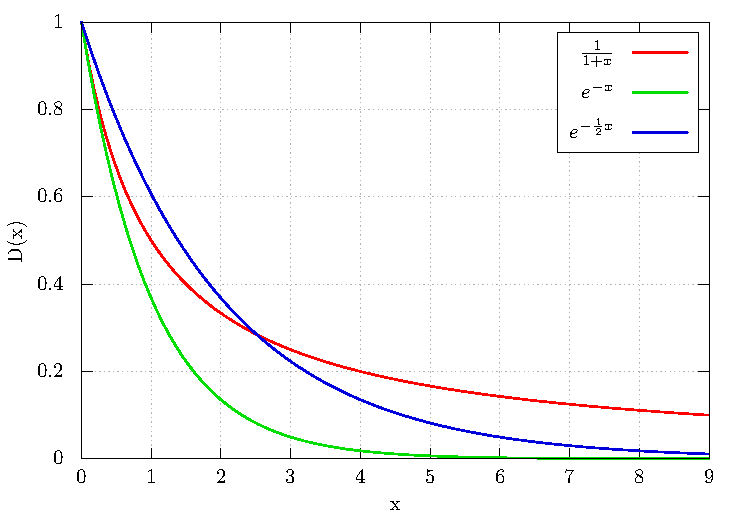
\includegraphics[scale=0.65]{dist_funcs.pdf}    
\end{frame}

\subsection{Surface}
\subsubsection{Solvent accesible surface}
\begin{frame}{Solvent accesible surface}
\end{frame}

\subsubsection{Evenly distributed points}
\begin{frame}{Evenly distributed points}
    \centering
    How to distribute $N$ points on a surface of a sphere?\\ ~\\ ~\\
    \raggedright
	\includesvg[scale=.2]{sphere_wireframe_coords}
\end{frame}

\subsubsection{Integration}
\begin{frame}{Integration}
\end{frame}

\end{document}
